\documentclass[thesis-solanki.tex]{subfiles}


\begin{document}

\chapter{Prototype 2.1}{\label{proto2.1}}

\section{About this chapter}
This chapter attempts to infuse the generic methodology from \ref{proto1} in a current \progLang{Prolog} implementation \cite{prolog-lib}
and make the unification "monadic".

\section{How prolog-0.2.0.1 works}

As described in the previous chapter about extending languages to incorporate functionality, this prototype applies the procedure to the
eDSL in \cite{prolog-lib}. 

The original abstract syntax used by the library,

\begin{minted}[linenos]{haskell}

data VariableName = VariableName Int String
      deriving (Eq, Data, Typeable, Ord)

type Atom         = String

data Term = Struct Atom [Term]
          | Var VariableName
          | Wildcard -- Don't cares 
          | Cut Int
      deriving (Eq, Data, Typeable)

data Clause = Clause { lhs :: Term, rhs_ :: [Goal] }
            | ClauseFn { lhs :: Term, fn :: [Term] -> [Goal] }
      deriving (Data, Typeable)

type Goal         = Term
type Program      = [Clause]
\end{minted} 

From the above we will focus on the \textit{Term} since the others just add wrappers around expressions which can be created by it. 

The implementation consists of components that one would find in a Language Processing System \ref{fig:A language-processing system},

\begin{figure}[th]
\centering
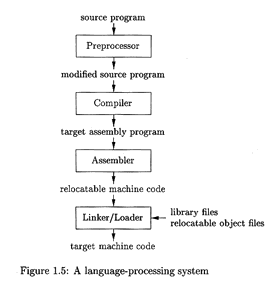
\includegraphics[scale = 0.7]{Language_Processing_System.png}
\caption{A language-processing system \cite{Aho:1986:CPT:6448}}
\label{fig:A language-processing system}
\end{figure}  

specifically speaking, parts of a compiler \ref{fig:Phases of Compiler},

\begin{figure}[th]
\centering
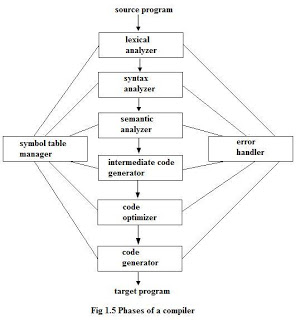
\includegraphics[scale = 0.7]{Phases_of_compiler.jpg}
\caption{Phases of Compiler \cite{Aho:1986:CPT:6448}}
\label{fig:Phases of Compiler}
\end{figure}  



The above language suffers from most of the problems discussed in the previous chapter.

The above is used to construct \progLang{Prolog} "terms" which are of a "single type".   

A database is used to store the terms which can then be used to resolve a query.

An interpreter to solve a query and lastly the unifier,

 


There are a few other components such as the REPL, Parser. 



\section{What we do in this prototype?}
In the first prototype we just did unification of two terms not query resolution.

We do complete \progLang{Prolog} query resolution like stuff.

\ref{proto1} provides a generic procedure / methodology to convert a language into monadic unifiable form 


\section{Current implementation (prolog-0.2.0.1)}
The current unification uses basic pattern matching to unfiy the terms 


\begin{minted}[linenos]{haskell}
unify, unify_with_occurs_check :: MonadPlus m => Term -> Term 
-> m Unifier

unify = fix unify'

unify_with_occurs_check =
   fix $ \self t1 t2 -> if (t1 `occursIn` t2 || t2 `occursIn` t1)
                           then fail "occurs check"
                           else unify' self t1 t2
 where
   occursIn t = everything (||) (mkQ False (==t))

unify' :: MonadPlus m => (Term -> Term -> m Unifier) -> Term -> 
Term -> m [(VariableName, Term)]

-- If either of the terms are don't cares then no unifiers exist
unify' _ Wildcard _ = return []
unify' _ _ Wildcard = return []

-- If one is a variable then equate the term to its value which 
-- forms the unifier
unify' _ (Var v) t  = return [(v,t)]
unify' _ t (Var v)  = return [(v,t)]

-- Match the names and the length of their parameter list and 
-- then match the elements of list one by one. 
unify' self (Struct a1 ts1) (Struct a2 ts2) 
            | a1 == a2 && same length ts1 ts2 = 
            unifyList self (zip ts1 ts2)

unify' _ _ _ = mzero

same :: Eq b => (a -> b) -> a -> a -> Bool
same f x y = f x == f y

-- Match the elements of each of the tuples in the list. 
unifyList :: Monad m => (Term -> Term -> m Unifier) -> 
[(Term, Term)] -> m Unifier
unifyList _ [] = return []
unifyList unify ((x,y):xys) = do
   u  <- unify x y
   u' <- unifyList unify (Prelude.map (both (apply u)) xys)
   return (u++u')
\end{minted} 


\section{Modifications}

The first modification is to the language is to make it compatible with the library whcih provides this nice generic mechanism a perform 
unification in a mondic manner.

Fixing, flattening, creating necessary instances 
\begin{minted}[linenos]{haskell}
data FTS a = FS Atom [a] | FV VariableName | FW | FC Int 
                          deriving (Show, Eq, Typeable, Ord)

newtype Prolog = P (Fix FTS) deriving (Eq, Show, Ord, Typeable) 

unP :: Prolog -> Fix FTS
unP (P x) = x 

instance Functor (FTS) where
  fmap              = T.fmapDefault

instance Foldable (FTS) where
  foldMap             = T.foldMapDefault

instance Traversable (FTS) where
    traverse f (FS atom xs)      =   FS atom <$> 
    sequenceA (Prelude.map f xs)
    traverse _ (FV v)          =   pure (FV v)
    traverse _ FW         =   pure (FW)
    traverse _ (FC i)          =   pure (FC i)

instance Unifiable (FTS) where
  zipMatch (FS al ls) (FS ar rs) = 
    if (al == ar) && (length ls == length rs) 
      then FS al <$> pairWith (\l r -> Right (l,r)) ls rs     
      else Nothing
  zipMatch FW _ = Just FW
  zipMatch _ FW = Just FW
  zipMatch (FC i1) (FC i2) = if (i1 == i2) 
    then Just (FC i1) 
    else Nothing

instance Applicative (FTS) where
  pure x                  =   FS "" [x] 
  _         <*>   FW    =   FW
  _       <*>   (FC i)     =   FC i
  _       <*>   (FV v)     = (FV v)
  (FS a fs) <*> (FS b xs)   = FS (a ++ b) [f x | f <- fs, x <- xs]
\end{minted}

some translation and helper functions .........

and finally the unification

\begin{minted}[linenos]{haskell}
monadicUnification :: (BindingMonad FTS (STVar s FTS) 
(ST.STBinding s)) 
=> (forall s. ((Fix FTS) -> (Fix FTS) -> 
  ErrorT (UT.UFailure (FTS) (ST.STVar s (FTS)))
           (ST.STBinding s) (UT.UTerm (FTS) (ST.STVar s (FTS)),
            Map VariableName (ST.STVar s (FTS)))))
monadicUnification t1 t2 = do
--  let
--    t1f = termFlattener t1
--    t2f = termFlattener t2
  (x1,d1) <- lift . translateToUTerm $ t1
  (x2,d2) <- lift . translateToUTerm $ t2
  x3 <- U.unify x1 x2
  --get state from somehwere, state -> dict
  return $! (x3, d1 `Map.union` d2)


goUnify ::
  (forall s. (BindingMonad FTS (STVar s FTS) (ST.STBinding s))
  =>
      (ErrorT
          (UT.UFailure FTS (ST.STVar s FTS))
          (ST.STBinding s)
          (UT.UTerm FTS (ST.STVar s FTS),
             Map VariableName (ST.STVar s FTS)))
     )
  -> [(VariableName, Prolog)]
goUnify test = ST.runSTBinding $ do
  answer <- runErrorT $ test --ERROR
  case answer of
    (Left _)            -> return []
    (Right (_, dict))   -> f1 dict


f1 ::
  (BindingMonad FTS (STVar s FTS) (ST.STBinding s))
  => (forall s. Map VariableName (STVar s FTS)
      -> (ST.STBinding s [(VariableName, Prolog)])
     )
f1 dict = do
  let ld1 = Map.toList dict
  ld2 <- Control.Monad.Error.sequence 
  [ v1 | (k,v) <- ld1, let v1 = UT.lookupVar v]
  let ld3 = [ (k,v) | ((k,_),Just v) <- ld1 `zip` ld2]
      ld4 = [ (k,v) | (k,v2) <- ld3, 
      let v = translateFromUTerm dict v2 ]
  return ld4
\end{minted}



\section{Results}

It works,

 

\end{document}
